In this chapter, we lay out the necessary background in graph theory for our later results. Section
\ref{sec:intro_graphs} includes fundamental definitions from graph theory and some important results
from spectral graph theory, while Section \ref{sec:small_world} introduces small world and scale-free
networks, which are graphs that have particular structural properties often found in real-world data.
Finally, Section \ref{sec:random_graphs} provides definitions relating to random graphs and relevant examples
of generative models.

\section{Elementary Graph Theory}
\label{sec:intro_graphs}

% two sentence summary of contents

% early on define complete, complete bipartite, and empty graphs under an
% example label

% recall \sum \lambda_i = \tr(M)

We begin by recalling some conventional definitions and notations from graph
theory.

\begin{definition}
  A \textbf{graph} $G$ is a pair of sets $(V,E)$ such that
  $E \subseteq \{ \{x,y\} | x,y \in V \}$. We call $V$ the set of
  \textbf{vertices} of $G$ and $E$ the set of \textbf{edges} of $G$.
\end{definition}


\begin{example}[The Pentagon]
  The \textbf{pentagon}, also known as the \textbf{5-cycle}, is the graph $(V,E)$ defined by
  $V = \{0,1,2,3,4\}$ and $E = \{\{0,1\}, \{1,2\}, \{2,3\},\allowbreak \{3,4\}, \{4,0\}\}$.
\end{example}

\begin{figure}[H]
  \centering
  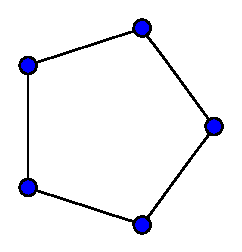
\includegraphics[width=0.25\textwidth]{pentagon.eps}
  \caption{The Pentagon}
  \label{fig:pentagon}
\end{figure}

\begin{remark}[Notation]
  Let $G = (V,E)$ be a graph.

  % reword access, ensure that these accessors are useful
  \begin{itemize}
  \item For convenience, we will use subscript notation to refer to the edge and vertex sets of $G$,
    i.e. $V_G = V$ and $E_G = E$.
  \item $v \in G$ is an equivalent statement to $v \in V_G$
  \item $|G|$, called the \textbf{order} of $G$, is equal to $|V_G|$.
  \end{itemize}
\end{remark}

When we speak about graphs, we are concerned with the structure of the graph
rather than the specific symbols in its vertex set. Thus we use the following
definition of equivalence.

\begin{definition}[Equivalence of graphs]
  Two graphs $G$ and $H$ are equivalent if there exists a bijection $\phi : V_G \to V_H$
  such that $\{u,v\} \in G$ if and only if $\{\phi(u),\phi(v)\} \in H$.
\end{definition}

Equivalence of graphs induces an equivalence relation on the set of all graphs. For convenience, we
will often only discuss graphs up to this equivalence relation (which only affects vertex labels).

\begin{example}
  \label{ex:basic_graphs}
  The \textbf{empty graph} of order $n$ is the graph such that $|V| = n$ and $E
  = \varnothing$.

  The \textbf{complete graph} of order $n$, denoted $K_n$, is the graph containing every possible
  edge, so that $|E_{K_n}| = \frac{n(n-1)}{2}$.

  We say a graph is \textbf{bipartite} when there exists a bipartition of its vertex set such that
  there are no edges between vertices in the same part. The \textbf{complete bipartite graph},
  denoted $K_{n,m}$, is such a graph where the two partitions have cardinality $n$ and $m$
  respectively, and every pair of vertices in distinct partitions is joined by an edge.
\end{example}

\begin{figure}[H]
  \centering
  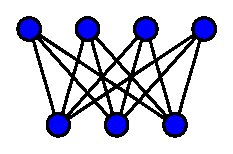
\includegraphics[width=0.4\textwidth]{k34.eps}
  \caption{The complete bipartite graph $K_{3,4}$}
  \label{fig:k34}
\end{figure}

\begin{definition}
  The \textbf{neighborhood} of a vertex $u \in G$, denoted $N(u)$, is the set of all vertices $v$
  such that $\{u,v\} \in E_G$, and these $v$ are called the neighbors of $u$. The \textbf{degree} of
  $u$ is defined by $\deg(u) = |N(u)|$. A graph in which every vertex has the same degree is
  \textbf{regular}. If that degree is equal to $k$, then the graph is said to be $k$-\textbf{regular}.
\end{definition}

\begin{example}
  $K_n$ is an $(n-1)$-regular graph, $K_{n,n}$ is an $n$-regular graph, and the pentagon is a
  $2$-regular graph.
\end{example}

\begin{definition}
  \label{def:walk_path}

  A \textbf{walk} of a graph $G$ is an alternating sequence of edges and vertices such that each
  vertex is incident to the edges before and after it.

  A \textbf{path} is the sequence of edges in a walk where every vertex is unique.

  The \textbf{shortest-path distance} between two vertices $u,v \in G$, denoted $\spd(u,v)$, is the
  minimum number of edges in a path from $u$ to $v$.
\end{definition}

\begin{definition}
  \label{def:adj_mat}
  The \textbf{adjacency matrix} $A$ of a graph $G$ is given by
  \[
    A_{ij} = \begin{cases}
      1 &: \{v_i,v_j\} ~\text{is an edge in $G$} \\
      0 &: \text{otherwise} \\
    \end{cases}
  \]

  where the set $\{v_i\}_{i=1}^{|G|}$ is an ordering of the vertices in $G$.
\end{definition}
 
%% Adjacency matrix properties
% - symmetric, (eigenvalues are real)
% - eigenvectors
% - spectral gap (+ defn)
% - example: k-regular graphs have largest (simple?) eigenvalue

Note that the adjacency matrix of a graph is not unique in general. Depending on
the way that the vertices of $G$ are numbered, we may end up with a different
matrix. However, for every adjacency matrix the following holds:


\begin{definition}
  A matrix is \textbf{reducible} if and only if it can be put in block upper triangular
  form by simultaneous row and column permutations. In other words, a matrix $M$
  is reducible if and only if there exists a permutation matrix $P$ such that
  $P^{-1}MP$ is block upper triangular. Otherwise, it is said to be
  \textbf{irreducible}.
\end{definition}

\begin{proposition}
  \label{prop:adj}
  Let $A$ be the adjacency matrix of a graph $G$. Then the following are true:

  \begin{enumerate}
  \item $A$ is symmetric (so the eigenvalues of $A$ are real)
  \item $A$ corresponds to a graph that is unique up to equivalence
  \item $A$ is irreducible if and only if $G$ is connected
  \end{enumerate}
\end{proposition}

\begin{proof}
  We omit proofs for (1) and (2) as they are self-evident.

  For (3), we first observe that $P^{-1}AP$ is an adjacency matrix of a graph
  equivalent to $G$ for any permutation matrix $P$. So without loss of generality, suppose that $G$ is
  connected and $A$ is already in block upper triangular form. Then because $A$
  is symmetric, we have

  \[
    A = \begin{bmatrix}
      B & \mathbf{0} \\
      \mathbf{0} & C
    \end{bmatrix}
  \]

  where $B$, $C$, are square block matrices. Say that $B$ has size $m \times m$. It is clear that
  there are no edges connecting the vertices in $\{1, ..., m\}$ to those in $\{m+1, ..., n\}$. Thus
  $G$ is not connected, which is a contradiction.
\end{proof}

The irreducibility result allows us to apply the Perron-Frobenius Theorem, resulting immediately in
these additional properties of $A$.

\begin{theorem}[Pg 673 (section 8.3) of ~\cite{alma991790573504746}]
  \label{thm:perron_frobenius}
  Let $A$ be an irreducible nonnegative square matrix of order $n$. The
  following is true.

  \begin{enumerate}
  \item Let $r$ be the maximum magnitude of the eigenvalues of $A$. Then $r$ is
    a (real, positive) simple eigenvalue of $A$.
  \item The eigenvalue $r$ has left and right eigenvectors whose components are
    all positive
  \item The only eigenvectors of $A$ whose components are all positive have
    eigenvalue $r$.
  \item
    \[ \min_i \sum_j a_{ij} \leq r \leq \max_i \sum_j a_{ij} \]
  \end{enumerate}
\end{theorem}

Because $A$ is nonnegative and irreducible for all connected graphs, these
properties hold for all such adjacency matrices. Indeed, the irreducibility and
nonnegativity of $A$ yields many other interesting properties which we omit
here.

\begin{definition}
  The \textbf{spectral gap} of a matrix $A$ is $\max_{i,j}|\lambda_i - \lambda_j|$, where
  $\lambda_i$ and $\lambda_j$ are the two largest eigenvalues of $G$.

  The \textbf{spectral gap of a graph} is the spectral gap of its adjacency matrix.
\end{definition}

We will next explore graph Laplacians, whose spectra are closely related to
those of adjacency matrices.

\begin{definition}
  \label{def:deg_mat}
  The \textbf{degree matrix} of $G$ is the diagonal matrix defined by
  \[
    D_{ij} = \begin{cases}
      \deg(i) &: i = j \\
      0 &: i \neq j
    \end{cases}
  \]
\end{definition}

\begin{definition}
  The \textbf{graph laplacian} of $G$ is given by $L = D - A$, where $D$ is the
  degree matrix of $G$ and $A$ is the adjacency matrix. In other words,

  \[
    L_{ij} = \begin{cases}
      \deg(i) &: i=j \\
      -1 &: (i,j) ~\text{is an edge in $G$} \\
      0 &: \text{otherwise}
    \end{cases}
  \]
\end{definition}

\begin{proposition}
  %%%%% \begin{enumerate}
  %%%%%   \item 
  %%%%% \end{enumerate}
  Let $G$ be a $k$-regular graph, $\{\lambda_i\}$ and $\{x_i\}$ be the sets of eigenvalues and
  eigenvectors for its adjacency matrix $A$, and $L$ be the graph Laplacian of $G$. Then
  \begin{enumerate}
  \item $\{\lambda_i - k\}$ is the eigenvalue set of $L$, and
  \item $\{x_i\}$ is the eigenvector set of $L$
  \item $L$ and $A$ have the same spectral gap
  \end{enumerate}
\end{proposition}

\begin{proof}
  Because $G$ is regular, the degree matrix $D$ is equal to $kI$. Let ant $x_i$ be given. Then
  \begin{align*}
    Lx_i &= (A-D)x_i \\
         &= \lambda_ix_i - kx_i \\
         &= (\lambda_i - k)x_i
  \end{align*}

  Which simultaneously shows (1) and (2). (3) follows trivially from (1).
\end{proof}

%% Graph laplacian discussion
% adjacency and eigenvalues relationship

% relationship between graph laplacian eigenvalues & spectracl gap

% eigenvalue distribution of A or L

% Wigner distribution for graph eigenvalues

% see random matrix theory "semicircle law"

% what happens when this is exponential?


\section{Small-World and Scale-free Networks}
\label{sec:small_world}

Small-world networks are a class of graphs characterized by having a very small
average shortest-path distance between any two vertices compared to the overall
size of the graph.

% eigenvalues and eigenvectors

\begin{definition}
  The \textbf{characteristic path length} of a graph $G = (V,E)$ is the average
  distance between vertices in the graph, which is given by

  \[ L_G = \frac{1}{|E|} \sum_{\substack{u,v \in V \\ u \neq v}} \dist(u,v)\]

  where $\dist(u,v)$ is shortest-path distance. 
\end{definition}

\begin{definition}[Page 1 of ~\cite{PhysRevLett.90.058701}]
  Consider a graph $G = (V,E)$. $G$ is a \textbf{small-world network} if
  $L_G \sim \log{|V|}$.
\end{definition}

Small-world networks are ubiquitous in a variety of applications areas. However, many real-world
examples of such graphs also have other distinctive structural properties which are not necessarily
captured by their small-worldedness alone ~\cite{Barabasi509}. Thus, we introduce the following
definition:


% We can partially describe this structure in terms of the
% clustering coefficient.

% \begin{definition}
%   Let $v$ be a vertex in a graph $G = (V,E)$.

%   Consider the subgraph formed by the neighborhood of $v$. This subgraph has at
%   most $\deg(v)(\deg(v) - 1)$ edges, which happens when it is a clique. Denote
%   the number of edges of the neighborhood subgraph by $E_{N(v)}$.

%   The \textbf{clustering coefficient} $C_v$ is defined by
%   $C_v = \frac{E_{N(v)}}{\deg(v)(\deg(v) - 1)}$, that is, $C_v$ is the
%   proportion of edges in the neighborhood subgraph out of all possible edges.
%   The clustering coefficient of $G$ is the average of all vertex clustering
%   coefficients, $C_G = \frac{\sum_{v \in V}{C_v}}{|V|}$.
% \end{definition}

\begin{definition}[Pg. 1 of ~\cite{PhysRevE.71.027103}]
  A \textbf{scale-free network} is a graph whose vertex degrees follow a power
  law. That is, given a randomly selected $u \in G$,
  $P(\deg(u) = k) \sim k^{-\gamma}$ for some $\gamma > 0$.
\end{definition}

One of the defining characteristics of power law distributions is that they have
very long tails. In a scale-free graph with many vertices, this implies the
existence of \textbf{hubs}, which we informally define as vertices whose degrees
are far larger than average in the graph.

Real world examples of scale-free networks are abundant and include the world
wide web, cellular communication networks, and protein-protein interaction (PPI)
networks. It is not surprising, then, that scale-free networks are necessarily
small-world networks, however we defer to Cohen and Havlin for proof of this
fact.

\begin{theorem}[Final result of ~\cite{PhysRevLett.90.058701}]
  Scale-free networks are small-world networks.
\end{theorem}



\section{Random Graphs}
\label{sec:random_graphs}

% exponential distribution eigenvalues

\begin{definition}
  A \textbf{random graph} is a random variable for which all outcomes are
  undirected graphs.

  A \textbf{random graph process}, denoted $(G_t)$, is a family of random graphs
  indexed by a discrete time $t \in \mathbb{N}$.
\end{definition}

We are interested in random graph processes which build small-world networks.
The Watts-Strogatz graphs are an example of such a process. They are defined by
starting with a regular ring lattice and randomly rewiring edges until the graph
is obtained.

\begin{definition}
  An $n$-$k$ \textbf{regular ring lattice} is a graph $(V, E)$ with $n$ vertices
  such that $u,v$ is an edge if and only if $|u-v| \leq \frac{k}{2}$.
\end{definition}

\begin{definition}
  Let $v$ be a vertex in a graph. We can \textbf{rewire} $v$ by deleting one
  edge of $v$ and drawing a new one by sampling uniformly from all vertices that
  do not share an edge with $v$.
\end{definition}

\begin{definition}
  Given a probability $p$ and regular ring lattice parameters $n$ and $k$, we
  define the $(n,k,p)$ \textbf{Watts-Strogatz Process} as follows.

  Let $r(G,v)$ be a random process that rewires vertex $v$ in a graph $G$. We
  define a family of graphs, $(G_t)$, by

  \[
    G_{t+1} = \left\{
      \begin{array}{lc}
        r(G_t,t) &: X \leq p \\
        G_t &: X > p
      \end{array}
    \right.
  \]

  for $t = 1,\dots, |G|$, where $G_0$ is the $n$-$k$ regular ring lattice, and
  $X$ is a uniform random variable in the range $[0,1]$. That is, we iterate
  over the vertices of the ring lattice and rewire each one with probability
  $p$.

  We call graphs sampled from $G_{|n|}$ \textbf{Watts-Strogatz graphs}.
\end{definition}

Watts and Strogatz showed empirically that the Watts-Strogatz graphs are small-world networks for all
but extremely small values of $p$~\cite{Watts1998Collective}. However, in general, they are not scale
free networks~\cite{Barabasi509}, and thus do not show the structural characteristics of many
practical data sets.

% TODO: ask about restated definitions
\begin{definition}[Pg. 511 of ~\cite{Barabasi509}]
  \label{def:ba}
  Let any graph $G_0$ be given as well as some parameter $m$, $m \leq |G_0|$. We
  build the random graph $G_{t+1}$ by adding a new vertex to $G_t$ and
  connecting it to $m$ vertices of $G_t$ with probabilities proportional to the
  degree of each vertex. That is, the probability of adding an edge to a vertex
  $u$ is

  \[
    p_u = \frac{\deg(v)}{\sum_{v \in G_t} \deg(v)}
  \]

  on the first step, and this is done a total of m times without replacement.

  We call $(G_t)$ the $(G_o,m)$-\textbf{Barab\'asi-Albert (BA) process} and graphs
  sampled from $G_n$ $(G_o,m,n)$-\textbf{Barab\'asi-Albert (BA) graphs}.
\end{definition}

This type of model, where edges to a new vertex are drawn with non-uniform
probability, is known as \textbf{preferential attachment}.

\begin{theorem}[Pg. 511 of ~\cite{Barabasi509}]
  \textbf{Barab\'asi-Albert graphs} are scale-free
\end{theorem}

The scale-free-ness of BA graphs makes them an attractive model, as they are likely to have degree
distributions similar to those of many real data sets. In addition, BA graphs are guaranteed to be
connected.

%%% Local Variables:
%%% mode: latex
%%% TeX-master: "../Main"
%%% End:
